\section{Příklad 1}
% Jako parametr zadejte skupinu (A-H)
\prvniZadani{C}
\[
  U_{12} = U_{1} + U_{2} = 100 + 80 = 180V
\]
\[
  R_{56} = \displaystyle\frac{R_{5}R_{6}}{R_{5}+R_{6}}  = \displaystyle\frac{220 \cdot 720}{220 + 720} = 168.51063829787233 \Omega
\]
\[
  R_{78} = R_{7} + R_{8} = 260 + 180 = 440\Omega
\]
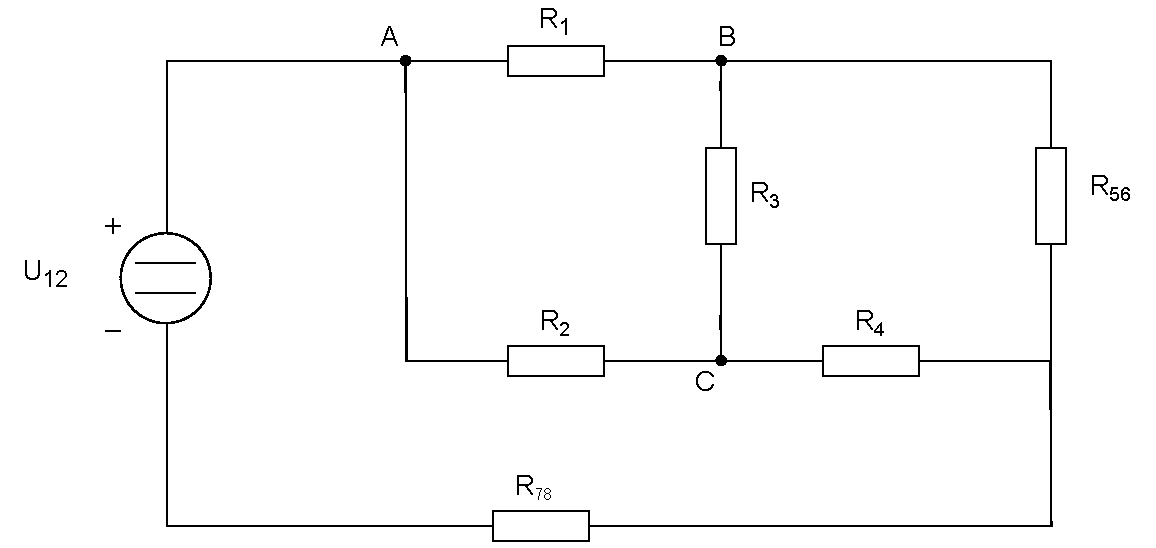
\includegraphics[scale=0.5,keepaspectratio]{fig/Pr1_1.pdf}\\
Nyní provedeme transfiguraci  trojuhelník hvězda
\[
  R_{A} = \displaystyle\frac{R_{1}R_{2}}{R_{1}+R_{2}+R_{3}}
  = \displaystyle\frac{450 \cdot 810}{450 + 810 + 190}
  = \displaystyle\frac{364500}{1450}
  = 251.37931034482768276 \Omega
\]
\[
  R_{B} = \displaystyle\frac{R_{1}R_{3}}{R_{1}+R_{2}+R_{3}}
  = \displaystyle\frac{450 \cdot 190}{450 + 810 + 190}
  = \displaystyle\frac{85500}{1450}
  = 58.96551724137931 \Omega
\]
\[
  R_{C} = \displaystyle\frac{R_{2}R_{3}}{R_{1}+R_{2}+R_{3}}
  = \displaystyle\frac{810 \cdot 190}{450 + 810 + 190}
  = \displaystyle\frac{153900}{1450}
  = 106.13793103448276 \Omega
\]
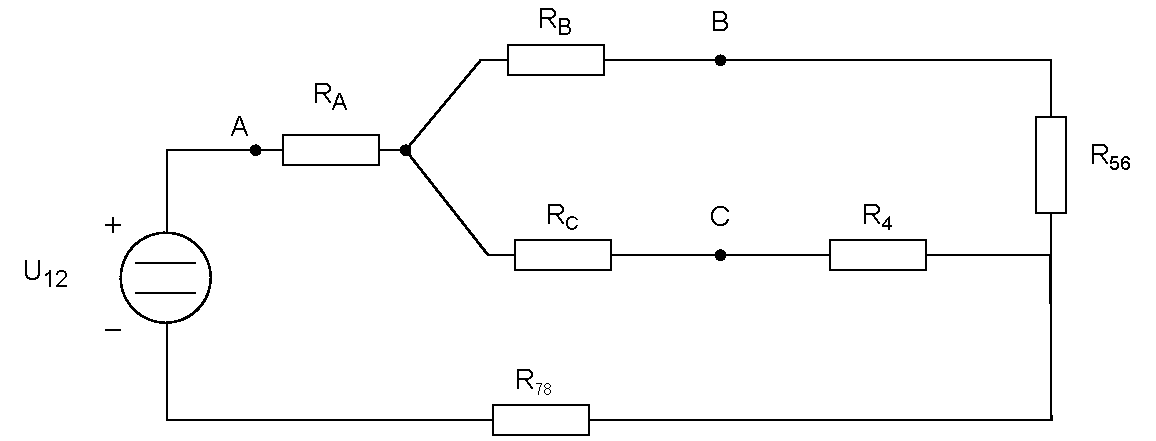
\includegraphics[scale=0.5,keepaspectratio]{fig/Pr1_2.pdf}
\[
  R_{B56} = R_{B} + R_{56} = 58.96551724137931 + 168.51063829787233 = 227.47615553925164 \Omega
\]
\[
  R_{C4} = R_{C} + R_{4} = 106.13793103448276 + 220 = 326.13793103448276 \Omega
\]
\[
  R_{B56C4} = \displaystyle\frac{R_{B56}R_{C4}}{R_{B56}+R_{C4}}
  = \displaystyle\frac{227.47615553925164 \cdot  326.13793103448276}{227.47615553925164 + 326.13793103448276}
  = 134.00779446635116 \Omega
\]
\[
  R_{EKV} = R_{A} + R_{B56C4} + R_{78} = 251.3793103448276 + 134.00779446635116 + 440
  = 825.3871048111787 \Omega
\]
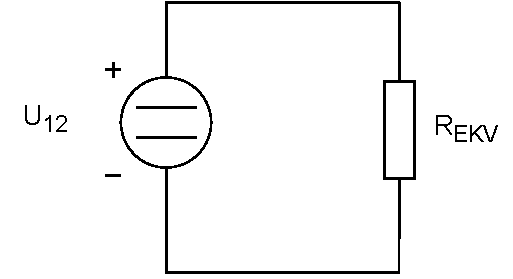
\includegraphics[scale=0.75,keepaspectratio]{fig/Pr1_4.pdf}\\
Celkový proud I
\[
  I = \displaystyle\frac{U}{R_{EKV}} = \displaystyle\frac{180}{825.3871048111787} = 0.21807949136929883A
\]
%\[
%  U_{AB5C4} = I \cdot (R_{B5C4} + R_A)\\
%  = 0.21807949136929883 \cdot (134.00779446635116  + 251.3793103448276)
 % = 84.04502379750852 V
%\]
\[
  U_{RA} = I \cdot R_A
  = 0.21807949136929883 \cdot 251.37931034482768276
  = 54.82067214076514V
\]
\[
  U_{B56C4} = I \cdot R_{B56C4}
 = 0.21807949136929883 \cdot 134.00779446635116
 = 29.224351656743398V
\]
\[
  I_{RC4} = \displaystyle\frac{U_{B56C4}}{R_{C4}} 
 = \displaystyle\frac{29.224351656743398}{326.13793103448276}
 = 0.08960733749688714 A
\] 
\[
  U_{RC} = I_{RC4} \cdot R_C
  = 0.08960733749688714  \cdot 106.13793103448276
  = 9.510737407428229 V
\]
\[
  U_{R2} = U_{RA} + U_{RC}
  = 9.510737407428229+54.82067214076514
  = \textbf{64.33140954819336V}
\]
\[
  I_{R2} = \displaystyle\frac{U_{R2}}{R_2}
  = \textbf{0.07942149326937452A}
\]

